\documentclass[doc, 12pt, a4paper, draftall]{apa7} % Document class

\usepackage{lipsum} % Generar texto ficticio Lorem Ipsum
\usepackage[american]{babel} % Configuración del idioma en español
\usepackage{csquotes} % Mejora las citas y referencias bibliográficas
\usepackage[style=apa,backend=biber]{biblatex} % Estilo APA para citas y referencias bibliográficas
\addbibresource{bibliography.bib} 
\usepackage{hyperref} % Creación de enlaces internos y externos en el documento PDF
\hypersetup{
    colorlinks=true, % Activar enlaces coloreados
    linkcolor=black, % Color de los enlaces internos (por defecto: red)
    citecolor=black, % Color de los enlaces de citas (por defecto: green)
    urlcolor=black, % Color de los enlaces URL (por defecto: magenta)
    linkbordercolor=white, % Color del borde de los enlaces internos (por defecto: red)
    citebordercolor=white, % Color del borde de los enlaces de citas (por defecto: green)
    urlbordercolor=white % Color del borde de los enlaces URL (por defecto: magenta)
}

%%%%%%%%% INCLUIR Y NUMERAR SECCIONES EN TOC Y DOCUMENTO %%%%%%%%%%%%%

\setcounter{tocdepth}{2} % Incluir hasta nivel de subsecciones en la tabla de contenidos
\setcounter{secnumdepth}{3} % Numerar hasta nivel de subsecciones
\AtBeginDocument{\addtocontents{toc}{\protect\thispagestyle{empty}}} % Desactivar numeración de página en la página de la tabla de contenidos

%%%%%%%%% AGREGAR PREFIJO A LOF Y LOT %%%%%%%%%%%%%
\usepackage{tocloft}

\renewcommand{\cftfigpresnum}{Figura }
\setlength{\cftfignumwidth}{5em}

\renewcommand{\cfttabpresnum}{Tabla }
\setlength{\cfttabnumwidth}{5em}

%%%%%%%%%% Centrado del título del ÍNDICE / LISTA DE FIGURAS / LISTA DE CUADROS %%%%%%%%%

\renewcommand{\cfttoctitlefont}{\hfill \normalfont\normalsize\bfseries}
\renewcommand{\cftaftertoctitle}{\hfill}

\renewcommand{\cftlottitlefont}{\hfill\normalfont\normalsize\bfseries}
\renewcommand{\cftafterlottitle}{\hfill}

\renewcommand{\cftloftitlefont}{\hfill\normalfont\normalsize\bfseries}
\renewcommand{\cftafterloftitle}{\hfill}

%%%%%%%%%% AGREGAR PREFIJO DE A SECCIONES Y A TOC %%%%%%%%%

\makeatletter
% Agregar prefijo a las secciones en la tabla de contenidos
%\renewcommand{\cftsecpresnum}{Capítulo }
%\renewcommand{\cftsecaftersnum}{:}
\setlength{\cftsecnumwidth}{6.5em}
\makeatother

\setlength{\cftbeforesecskip}{2mm}
\renewcommand\cftsecafterpnum{\vskip5pt}
\renewcommand\cftsubsecafterpnum{\vskip5pt}
\renewcommand\cftsubsubsecafterpnum{\vskip5pt}

%%%%%%%%%%%%%% DEFINIR INFORMACIÓN PERSONAL Y TRABAJO %%%%%%%%%%%%%%%%%%%%

%Título de la DOCUMENTO (Siempre en mayuscula y sin saltos de linea)
\title{PROPUESTA DE IMPLEMENTACIÓN DE UN REFORZAMIENTO ESTRUCTURAL PARA REDUCIR LA VULNERABILIDAD SÍSMICA DE LA IGLESIA VILLA DE HUAYLLAY USANDO MODELO DE ELEMENTOS FINITOS}

%Título corto del DOCUMENTO al pie de PÁGINA (Agregar salto de línea de ser necesario)
\shorttitle{PROPUESTA DE IMPLEMENTACIÓN DE UN REFORZAMIENTO ESTRUCTURAL PARA REDUCIR LA VULNERABILIDAD SÍSMICA DE LA IGLESIA VILLA DE HUAYLLAY USANDO MODELO DE ELEMENTOS FINITOS}

%Nombre de la FACULTAD (Siempre en mayuscula)
\faculty{FACULTAD DE INGENIERÍA}

%Para obtener el GRADO profesional de ...
\degree{Ingeniería Civil}

%AUTOR para carátula (Siempre en mayuscula y sin saltos de linea)
\authorname{SANCHEZ CARBAJAL, DINER ERICK}
\authororcid{(XXXX-XXXX-XXXX-XXXX)}

%ASESOR para carátula (Siempre en mayuscula y sin saltos de linea)
\advisorname{ING. SOTO OBLEA, EDWARD JONATHAN}
\advisororcid{(XXXX-XXXX-XXXX-0000)}

%AÑO para carátula
\yyearr{2023}
 % Call preamble using input

\begin{document}

% Carátula del documento
\maketitle

% Epígrafe
\begin{epigraph}
  \hfill {\fontsize{9}{13}\selectfont \hfill A mis queridos padres Edgar y Alberta, por  su apoyo, comprensión y concejos. A mis hermanos por alegrarme en los momentos más importantes de mi vida. A mis queridos padres Edgar y Alberta,  por  su apoyo concejos. A mis hermanos por alegrarme en los momentos más importa mi vida.} 
\end{epigraph}

\frontmatter % Comenzar numeración romana

% Tabla de contenidos
\renewcommand\contentsname{\centering Índice}
\tableofcontents
\newpage
\renewcommand\listtablename{\centering Índice de Tablas}
\listoftables
\newpage
\renewcommand\listfigurename{\centering Índice de Figuras}
\listoffigures
\newpage

\begin{dedication}
 \hfill {\fontsize{8}{13}\selectfont A mis queridos padres Edgar y Alberta,  por  su apoyo, comprensión  y  concejos. A mis hermanos por alegrarme en los momentos más importantes de mi vida.}
\end{dedication}
  
\begin{acknowledgments}
  Agradecimientos aquí
\end{acknowledgments}
  
\begin{resumen}
  Resumen aquí
\end{resumen}
  
\begin{abstract}
  Abstract here
\end{abstract}

\mainmatter % Comenzar numeración arábica

\section{Introducción}

\lipsum[2]

\section{Planteamiento del Problema}

\subsection{Situación Problemática}

\begin{figure}[!ht]
	\centering
  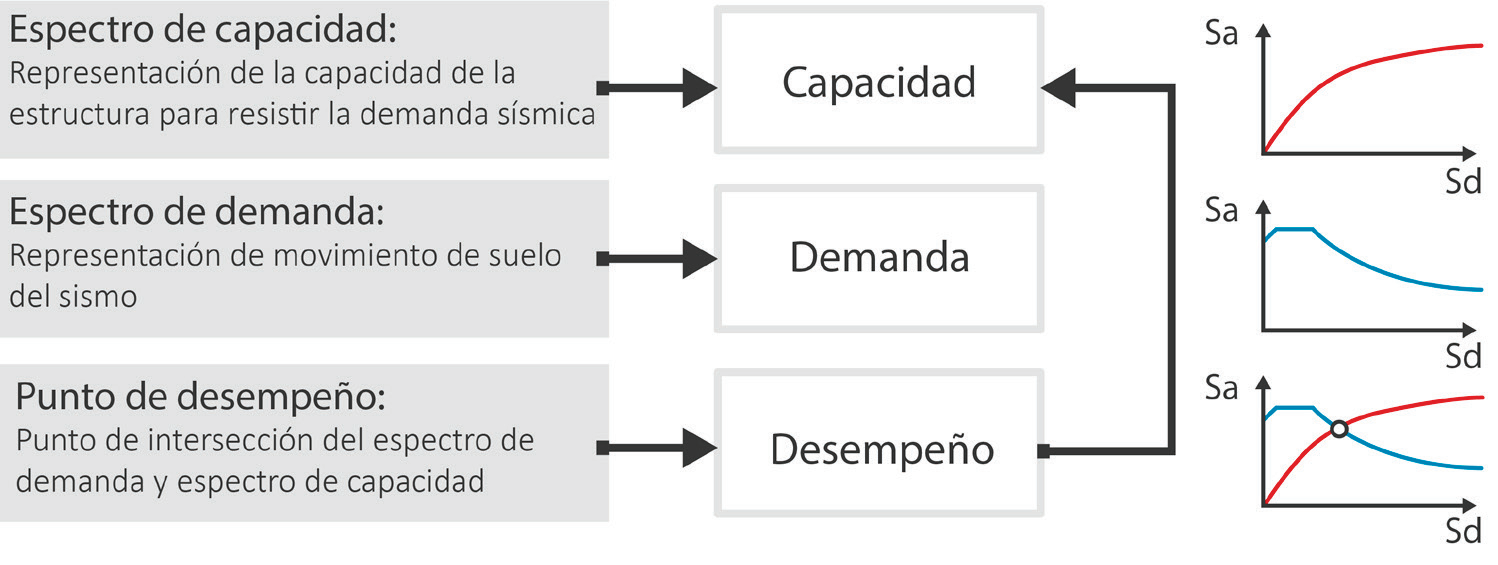
\includegraphics[scale=0.36]{E_IMAGENES/3_Capitulo3/Cap3_Imagen70.png}
	\caption{\centering\footnotesize Cuadro y gráficos que muestran el método N2. Adaptado de \cite{deWaal2009}}
  \figurenote{This is a great figure.}
	\label{Cap3_Figura8}
\end{figure}

\Textcite{vonDavier2011} said this, that
too \parencite{vonDavier2011,Lassen2006}.  Further evidence comes from
other sources \parencite{Shotton1989,Lassen2006}.  

\lipsum[3]

\lipsum[4]

\subsection{Formulación del Problema}

\lipsum[5]

\subsection{Justificación de la Investigación}

\lipsum[6]

\subsection{Objetivos de la Investigación}

\lipsum[7]

\subsubsection{Objetivo General}

\lipsum[8]

\subsubsection{Objetivos Específicos}

\lipsum[9]

\subparagraph{Inter-rater reliability}
\lipsum[10]

\subparagraph{Test-retest reliability}
\lipsum[11]

\paragraph{Validity}
\lipsum[12]

\subparagraph{Face validity}
\lipsum[13]

\subparagraph{Construct validity}
\lipsum[14]

\section{Marco Teórico}

\subsection{Antecendentes del Problema}

\lipsum[15]

\lipsum[15]

\subsection{Bases Teóricas}

\lipsum[2]

\subsection{Marco Conceptual}

Table~\ref{tab:BasicTable} summarizes the data. \lipsum[15]

\begin{table}
  \caption{Sample Basic Table}
  \label{tab:BasicTable}
  \begin{tabular}{@{}llr@{}}         \toprule
  \multicolumn{2}{c}{Item}        \\ \cmidrule(r){1-2}
  Animal    & Description & Price \\ \midrule
  Gnat      & per gram    & 13.65 \\
            & each        &  0.01 \\
  Gnu       & stuffed     & 92.50 \\
  Emu       & stuffed     & 33.33 \\
  Armadillo & frozen      &  8.99 \\ \bottomrule
  \end{tabular}
\end{table}

\begin{figure}[!ht]
	\centering
  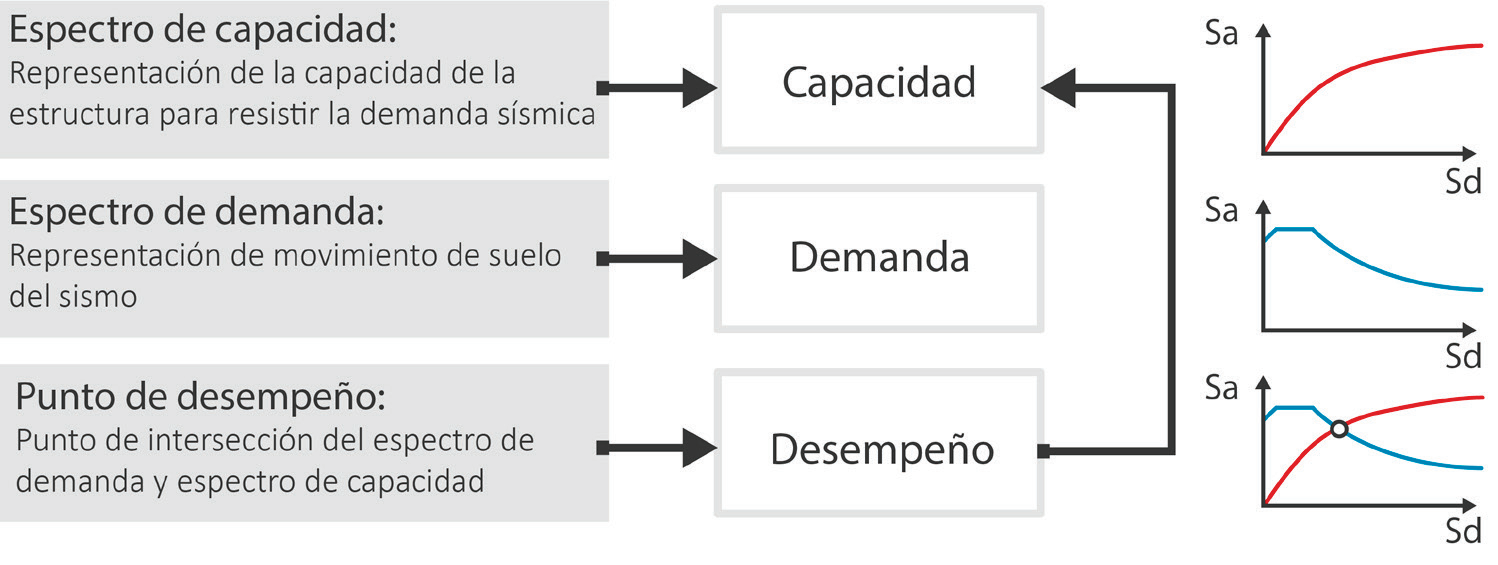
\includegraphics[scale=0.36]{E_IMAGENES/3_Capitulo3/Cap3_Imagen70.png}
	\caption{\centering\footnotesize Cuadro y gráficos que. Adaptado de \cite{deWaal2009}}
  \figurenote{This is a great figure.}
	\label{Cap3_Figura2}
\end{figure}

Figure~\ref{Cap3_Figura8} shows this trend. \lipsum[16]

\section{Hipótesis y Variables}

\subsection{Hipótesis General}

\subsection{Hipótesis Específicas}

\subsection{Identificación de Variables}

\subsection{Operacionalización de Variables}

\subsection{Matriz de Consistencia}

\lipsum[17]

\lipsum[18]

\begin{figure}[!ht]
	\centering
  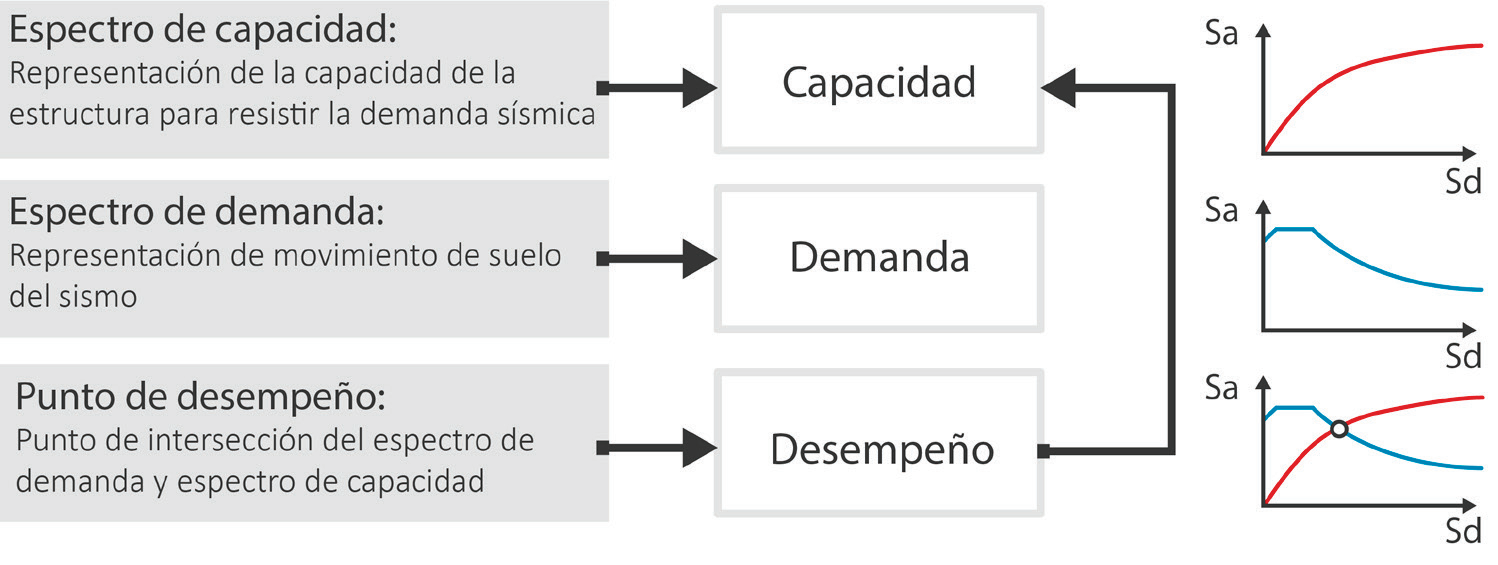
\includegraphics[scale=0.36]{E_IMAGENES/3_Capitulo3/Cap3_Imagen70.png}
	\caption{\centering\footnotesize Cuadro y gráficos que muestran el método N2. Adaptado de \cite{deWaal2009}}
  \figurenote{This is a great figure.}
	\label{Cap3_Figura3}
\end{figure}

\lipsum[19]

\section{Metodología}

\subsection{Tipo y Diseño de Investigación}

\subsection{Unidad de Análisis}

\subsection{Población de Estudio}

\subsection{Tamaño de Muestra}

\subsection{Selección de Muestra}

\subsection{Técnicas e Instrumentos de Recolección de Datos}

\subsection{Análisis e Interpretación de la Información}

\section{Procedimiento y Método de Análisis}

\subsection{Iglesia Villa de Huayllay}

\subsection{Obtención de datos}

\subsection{Implementación MEF}

\subsection{Calibración MEF}

\subsection{Evaluación de la Vulnerabilidad Sísmica sin Refuerzo}

\subsection{Propuesta de Reforzamiento Estructural}

\subsection{Evaluación de la Vulnerabilidad Sísmica con Refuerzo}


\backmatter % Continuar numeración arábica

\printbibliography[heading=bibintoc, title={Referencias}]

\appendix

\section{Instrument}
\label{app:instrument}

As shown in Figure~\ref{fig:Figure2}, these results are impressive. \lipsum[20]

\begin{figure}[!ht]
	\centering
  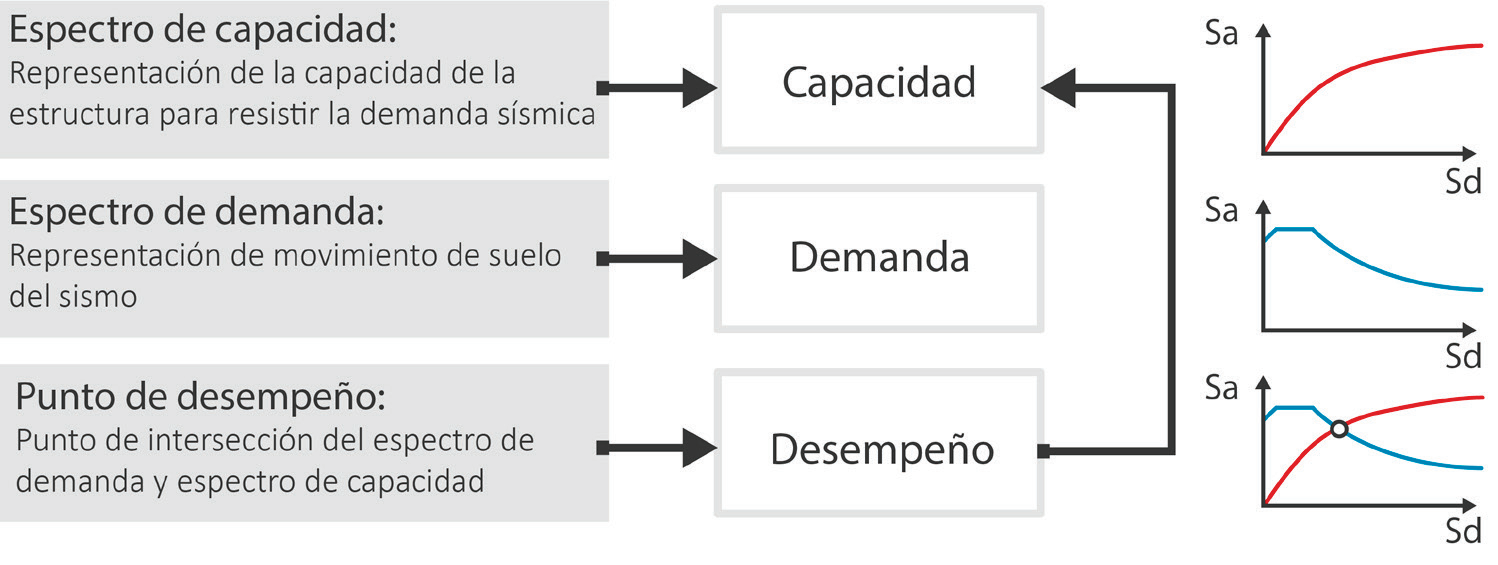
\includegraphics[scale=0.36]{E_IMAGENES/3_Capitulo3/Cap3_Imagen70.png}
	\caption{\centering\footnotesize Cuadro y gráficos que muestran el método N2. Adaptado de \cite{deWaal2009}}
  \figurenote{\centering\footnotesize This is a great figure.}
	\label{fig:Figure2}
\end{figure}

\lipsum[21]
\section{Pilot Data}
\label{app:surveydata}

The detailed results are shown in Table~\ref{tab:DeckedTable} from Anexo~\ref{app:surveydata}.

\lipsum[22]

\begin{table}
  \begin{threeparttable}
    \caption{A More Complex Decked Table}
    \label{tab:DeckedTable}
    \begin{tabular}{@{}lrrr@{}}         \toprule
    Distribution type  & \multicolumn{2}{l}{Percentage of} & Total number   \\
                       & \multicolumn{2}{l}{targets with}  & of trials per  \\
                       & \multicolumn{2}{l}{segment in}    & participant    \\ \cmidrule(r){2-3}
                                    &  Onset  &  Coda            &          \\ \midrule
    Categorical -- onset\tabfnm{a}  &    100  &     0            &  196     \\
    Probabilistic                   &     80  &    20\tabfnm{*}  &  200     \\
    Categorical -- coda\tabfnm{b}   &      0  &   100\tabfnm{*}  &  196     \\ \midrule
    \end{tabular}
    \tablenote{All data are approximate.

            \tabfnt{a}Categorical may be onset.
            \tabfnt{b}Categorical may also be coda.

            \tabfnt{*}\textit{p} < .05.
            \tabfnt{**}\textit{p} < .01.
         }
  \end{threeparttable}
\end{table}

\lipsum[23]

\end{document}

% 
% Copyright (C) 2022 by Daniel A. Weiss <daniel.weiss.led at gmail.com>
% 
% This work may be distributed and/or modified under the
% conditions of the LaTeX Project Public License (LPPL), either
% version 1.3c of this license or (at your option) any later
% version.  The latest version of this license is in the file:
% 
% http://www.latex-project.org/lppl.txt
% 
% Users may freely modify these files without permission, as long as the
% copyright line and this statement are maintained intact.
% 
% This work is not endorsed by, affiliated with, or probably even known
% by, the American Psychological Association.
% 
% 
% This work is "maintained" (as per LPPL maintenance status) by
% Daniel A. Weiss.
% 
% This work consists of the file  apa7.dtx
% and the derived files           apa7.ins,
%                                 apa7.cls,
%                                 apa7.pdf,
%                                 README,
%                                 APA7american.txt,
%                                 APA7british.txt,
%                                 APA7dutch.txt,
%                                 APA7english.txt,
%                                 APA7french.txt,
%                                 APA7german.txt,
%                                 APA7ngerman.txt,
%                                 APA7greek.txt,
%                                 APA7czech.txt,
%                                 APA7turkish.txt,
%                                 APA7spanish.txt,
%                                 APA7hungarian.txt,
%                                 APA7endfloat.cfg,
%                                Figure1.pdf,
%                                 shortsample.tex,
%                                 longsample.tex, and
%                                 bibliography.bib.